% Hetedik előadás

\chapter{Lebegőpontos és BCD számok}

\section{Bevezetés}
A lebegőpontos számok szükségesek, mivel:
\begin{itemize}
    \item a fixpontos számok értelmezési tartománya viszonylag kicsi
    \item fixpontos számoknál a pontosság is viszonylag kicsi
\end{itemize}

A lebegőpontos számokat 1985-ben szabványosították (IEE754).
Formájuk: $M*r^k$, ahol M a mantissza, r a radix és k a karakterisztika.
Fontos, hogy r alapja megegyezzen az M számrendszerének alapjával.

\section{Ábrázolás}
A lebegőpontos számok ábrázolása normalizált formátumban történik, tehát a tizedes (kettes számrendszernél kettedes) pont után következik az első értékes számjegy.
Példa: $0,1011*2^k$.

\section{A mantissza lehetséges értékei}
Ezzel a mantissza értéke fix intervallumba kerül, pl. 10-es számrendszernél $0,1 <= M < 1$.
Ugyanez általánosan megfogalmazva: $1/r <= M < 1$.

\section{Értelmezési tartomány}
A lebegőpontos számok értelmezési tartománya függ:
\begin{itemize}
    \item a karakterisztika számára rendelkezésre álló bitek számától
    \item a radixtól
\end{itemize}

\section{Pontosság}
Példa: $0,3014*10^6$.
Ekkor ha a mantisszára 3 bitet allokálunk, elveszítjük a 4-es számjegyet, csökken a pontosság.
A pontosság tehát függ a mantissza hosszától (rendelkezésre álló bitek számától).

\section{Alulcsordulás és túlcsordulás}
Az értelmezési tartományon kívül eső értékeket nem tudjuk ábrázolni, így ott túlcsordulás keletkezik.
Mivel a mantisszának 0,1-nél nagyobb vagy egyenlőnek kell lennie, ezért a nullát sem tudjuk ábrázolni, alulcsordulás keletkezik.
Az alul- és túlcsordulási régiók nagysága elsősorban a karakterisztikára allokált bitektől függ.
\begin{figure}[H]
    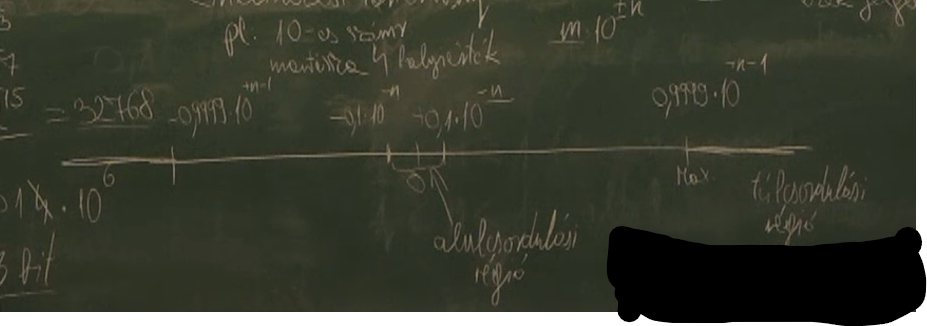
\includegraphics[width=0.8\textwidth]{csord}
    \centering
    \caption{Alul- és túlcsordulási régiók}
    \label{fig:csord}
\end{figure}

Az architektúrának biztosítania kell a túlcsordulás felismerését, jelzését és kezelését.

Az architektúra lehetőségei túlcsordulás esetén:
\begin{itemize}
    \item kijelzi a túlcsordulást és beállítja a legnagyobb megengedett értéket
    \item kijelzi a túlcsordulást és előjeles végtelent jelez ki
\end{itemize}
Alulcsordulás esetén:
\begin{itemize}
    \item kijelzi az alulcsordulást és nullára konvertál
    \item kijelzi az alulcsordulást denormalizált számot jelzi ki
\end{itemize}
A kijezést flagek segítségével teszi.

A szabvány előírja, hogy ha a mantissza nulla, a karakterisztikának is nullának kell lennie.

\section{Pontosság növelése}
Probléma, hogy a tízes számrendszerben pontosan megadható számok egy része kettes számrendszerben végtelen tizedes törtként ábrázolható (pl. 0.3).
A pontosság növelésére alkalmazott módszerek:
\begin{itemize}
    \item rejtett bit használata: a mantissza tört utáni részénél az első számjegy (bit) mindig 1, így nincs információtartalma. Ezért azt nem tároljuk, így egy bittel pontosabb számot tudunk tárolni.
    \item őrző bitek: a szabvány elvárása, hogy a pontatlanság kisebb legyen, mint a normalizált eredmény legkisebb számjegye. Probléma, hogy normalizáláskor értékes biteket veszíthetünk el, ezért a CPU-n belül a regiszterek több biten tárolják a mantisszát. Általában +3-15 bit. Ezek az őrző bitek, amik a memóriában tárolás során nem jelennek meg. Az őrző bitek felhasználása:
    \begin{itemize}
        \item a rejtett bit balra léptetésekor értékes bitet tudunk beléptetni
        \item tárolási formátum kérésekor kerekített értéket tárolhatunk
        \item normalizáláskor értékes biteket tudunk felhasználni
    \end{itemize}
\end{itemize}

\section{Lebegőpontos műveletvégzés jellemzői}
\begin{itemize}
    \item kódolás: mantissza kódolása 2-es komplemens, karakterisztika kódolása többletes kódolással. Ennek oka, hogy a többletes kód kialakítása gyorsabb, de elsősorban csak összeadás és kivonás elvégzésére alkalmas. Szorzást, osztást egyszerűbb kettes komplemenssel kódolt számokon könnyebb.
\end{itemize}

\section{IEEE 754 további jellemzői}
A szabvány fő célja a kompatibilitás megteremtése különböző CPU-k között.
A hardvernek és a szoftvernek együtt kell biztosítania a szabványnak való megfelelést.

A szabvány legfontosabb fejezetei:
\begin{itemize}
    \item adattípus
    \item formátumok
    \begin{itemize}
        \item szabványos (háttértáron tárolás)
        \begin{itemize}
            \item egyszeres pontosságú (32 bit)
            \item kétszeres pontosságú (64 bit)
        \end{itemize}
        \item kiterjesztett (CPU-n belül)
        \begin{itemize}
            \item egyszeres pontosságú (32 bit)
            \item kétszeres pontosságú (64 bit)
        \end{itemize}
    \end{itemize}
    \item műveletek
    \item kerekítések
    \item kivételek kezelése
\end{itemize}

A szabvány által meghatározott műveletek:
\begin{itemize}
    \item négy aritmetikai művelet
    \item maradékképzés
    \item gyökvonás
    \item bináris-decimális konverzió
    \item értelmezett a végtelennel való műveletvégzés
    \item kerekítések
    \begin{itemize}
        \item legközelebbire kerekítés
        \item nullára kerekítés (őrző bitek levágása)
        \item kerekítés pozitív végtelen felé
        \item kerekítés negatív végtelen felé
    \end{itemize}
\end{itemize}

A kivételek felbukkanása általában megszakítást eredményez.
Kivételek lehetnek pl. overflow, underflow, nullával osztás, gyökvonás negatív számból.

Először a lebegőpontos egységek koprocesszorokban voltak, később az Intel 80486 CPU-nál már a processzorba volt integrálva.

\section{Műveletek megvalósítása}

\begin{itemize}
    \item A+B: azonos hatványra hozás és összeadás
    \item A*B: A és B mantisszájának szorzása és a karakterisztikák összeadása
\end{itemize}
A szorzásnál fontos, hogy a két művelet párhuzamosan elvégezhető, így növelhető a sebesség.
Ennek a megvalósítása dedikált FP műveletvégzővel történik: egy adatbuszon keresztül a mantissza a mantissza egységbe, a karakterisztika pedig a karakterisztika egységbe kerül, a végeredményt pedig a vezérlő rakja össze.

\section{BCD számábrázolás}
Megjelenésének fő oka a fixpontos és a lebegőpontos számok pontatlansága.
Elsősorban adminisztratív és tudományos alkalmazásoknál használják (pl. számológépek).
A lebegőpontos konvertálás lehet pontatlan, de a kódolás pontos megfeleltetés, nincs kerekítés.

BCD kódolásnál minden számjegyet 4 biten ábrázolunk.
Mivel 4 bit 16 féle értéket vehet fel, keletkezik 6 darab érvénytelen tetrád, ami nincs használatban BCD kódolásnál.

\subsection{Ábrázolási formátumok}
\begin{itemize}
    \item zónázott: 1 byte = 1 számjegy, minden tetrádot megelőz 4 zóna bit
    \item pakolt: 1 byte = 2 számjegy (pl. Intel)
\end{itemize}

\subsection{Műveletvégzés logikai szinten}
Példa: 8+7=15.
BCD kódolva ez 1000+0111=1111, ami egy érvénytelen tetrádot eredményez, így 10-et ki kell vonni belőle (azaz hozzáadunk -10-et).
Kettes komplemens esetben 1010 invertálva 0101, majd hozzáadva egyet 0110.
Ezzel előáll az 5 mint eredmény.

\subsection{Műveletvégzés áramköri szinten}
A megvalósításhoz szükség van 4 db teljes összeadóra.
Az áramkörnek el kell végeznie az érvénytelen tetrádok kezelését is.
Az előző példánál az áramkör működése:
\begin{figure}[H]
    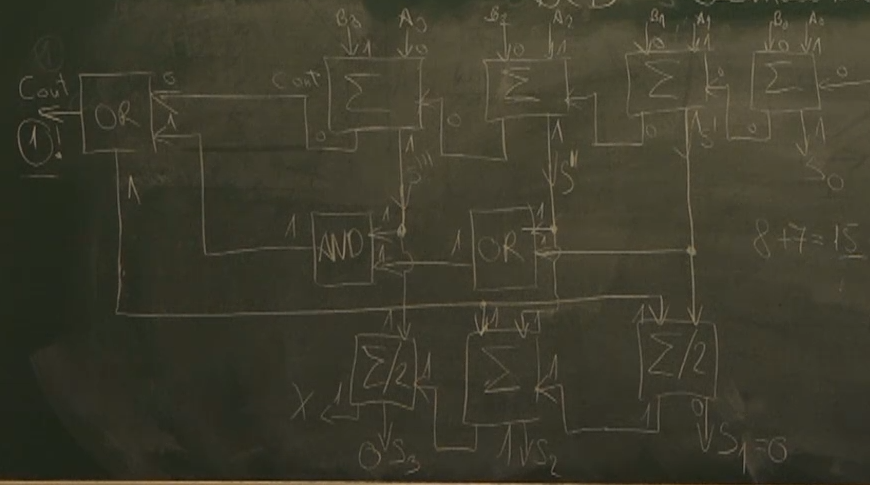
\includegraphics[width=0.8\textwidth]{bcd}
    \centering
    \caption{BCD összeadó áramkör}
    \label{fig:bcd}
\end{figure}

\subsection{Összegzés}
A BCD kódolás előnye tehát, hogy teljesen pontos, viszont jelentősen több helyet foglal, mint a lebegőpontos számok, valamint lassabb a végrehajtás is sok esetben.
A BASIC programnyelv ezt használja.

\section{Az ALU egyéb műveletei}
Az aritmetikai műveleteken kívül egyéb műveleteket is ellát az ALU, ezek általában egyszerűbb áramköröl segítségével megoldhatók.
\begin{itemize}
    \item Boole műveletek (mind a 16 fajta) pl.:
    \begin{itemize}
        \item AND
        \item NOR
        \item XOR
    \end{itemize}
    \item léptetés
    \item invertálás
    \item komparálás (feltételes ugrás)
    \item LOAD/STORE címszámítás - valós időben címet generál a MAR számára
    \item karakteres műveletek
\end{itemize}